
%% bare_conf.tex
%% V1.4b
%% 2015/08/26
%% by Michael Shell
%% See:
%% http://www.michaelshell.org/
%% for current contact information.
%%
%% This is a skeleton file demonstrating the use of IEEEtran.cls
%% (requires IEEEtran.cls version 1.8b or later) with an IEEE
%% conference paper.
%%
%% Support sites:
%% http://www.michaelshell.org/tex/ieeetran/
%% http://www.ctan.org/pkg/ieeetran
%% and
%% http://www.ieee.org/

%%*************************************************************************
%% Legal Notice:
%% This code is offered as-is without any warranty either expressed or
%% implied; without even the implied warranty of MERCHANTABILITY or
%% FITNESS FOR A PARTICULAR PURPOSE! 
%% User assumes all risk.
%% In no event shall the IEEE or any contributor to this code be liable for
%% any damages or losses, including, but not limited to, incidental,
%% consequential, or any other damages, resulting from the use or misuse
%% of any information contained here.
%%
%% All comments are the opinions of their respective authors and are not
%% necessarily endorsed by the IEEE.
%%
%% This work is distributed under the LaTeX Project Public License (LPPL)
%% ( http://www.latex-project.org/ ) version 1.3, and may be freely used,
%% distributed and modified. A copy of the LPPL, version 1.3, is included
%% in the base LaTeX documentation of all distributions of LaTeX released
%% 2003/12/01 or later.
%% Retain all contribution notices and credits.
%% ** Modified files should be clearly indicated as such, including  **
%% ** renaming them and changing author support contact information. **
%%*************************************************************************


% *** Authors should verify (and, if needed, correct) their LaTeX system  ***
% *** with the testflow diagnostic prior to trusting their LaTeX platform ***
% *** with production work. The IEEE's font choices and paper sizes can   ***
% *** trigger bugs that do not appear when using other class files.       ***                          ***
% The testflow support page is at:
% http://www.michaelshell.org/tex/testflow/



\documentclass[conference]{IEEEtran}
% Some Computer Society conferences also require the compsoc mode option,
% but others use the standard conference format.
%
% If IEEEtran.cls has not been installed into the LaTeX system files,
% manually specify the path to it like:
% \documentclass[conference]{../sty/IEEEtran}


\usepackage[usenames,dvipsnames]{color}
\newcommand{\todo}[1]
  {{\scriptsize \textbf{\color{red} {#1}}}}



% Some very useful LaTeX packages include:
% (uncomment the ones you want to load)


% *** MISC UTILITY PACKAGES ***
%
%\usepackage{ifpdf}
% Heiko Oberdiek's ifpdf.sty is very useful if you need conditional
% compilation based on whether the output is pdf or dvi.
% usage:
% \ifpdf
%   % pdf code
% \else
%   % dvi code
% \fi
% The latest version of ifpdf.sty can be obtained from:
% http://www.ctan.org/pkg/ifpdf
% Also, note that IEEEtran.cls V1.7 and later provides a builtin
% \ifCLASSINFOpdf conditional that works the same way.
% When switching from latex to pdflatex and vice-versa, the compiler may
% have to be run twice to clear warning/error messages.






% *** CITATION PACKAGES ***
%
%\usepackage{cite}
% cite.sty was written by Donald Arseneau
% V1.6 and later of IEEEtran pre-defines the format of the cite.sty package
% \cite{} output to follow that of the IEEE. Loading the cite package will
% result in citation numbers being automatically sorted and properly
% "compressed/ranged". e.g., [1], [9], [2], [7], [5], [6] without using
% cite.sty will become [1], [2], [5]--[7], [9] using cite.sty. cite.sty's
% \cite will automatically add leading space, if needed. Use cite.sty's
% noadjust option (cite.sty V3.8 and later) if you want to turn this off
% such as if a citation ever needs to be enclosed in parenthesis.
% cite.sty is already installed on most LaTeX systems. Be sure and use
% version 5.0 (2009-03-20) and later if using hyperref.sty.
% The latest version can be obtained at:
% http://www.ctan.org/pkg/cite
% The documentation is contained in the cite.sty file itself.






% *** GRAPHICS RELATED PACKAGES ***
%
\ifCLASSINFOpdf
   \usepackage[pdftex]{graphicx}
  % declare the path(s) where your graphic files are
   \graphicspath{{images/}}
  % and their extensions so you won't have to specify these with
  % every instance of \includegraphics
   \DeclareGraphicsExtensions{.pdf,.jpeg,.png, .jpg}
\else
  % or other class option (dvipsone, dvipdf, if not using dvips). graphicx
  % will default to the driver specified in the system graphics.cfg if no
  % driver is specified.
  % \usepackage[dvips]{graphicx}
  % declare the path(s) where your graphic files are
  % \graphicspath{{../eps/}}
  % and their extensions so you won't have to specify these with
  % every instance of \includegraphics
  % \DeclareGraphicsExtensions{.eps}
\fi
% graphicx was written by David Carlisle and Sebastian Rahtz. It is
% required if you want graphics, photos, etc. graphicx.sty is already
% installed on most LaTeX systems. The latest version and documentation
% can be obtained at: 
% http://www.ctan.org/pkg/graphicx
% Another good source of documentation is "Using Imported Graphics in
% LaTeX2e" by Keith Reckdahl which can be found at:
% http://www.ctan.org/pkg/epslatex
%
% latex, and pdflatex in dvi mode, support graphics in encapsulated
% postscript (.eps) format. pdflatex in pdf mode supports graphics
% in .pdf, .jpeg, .png and .mps (metapost) formats. Users should ensure
% that all non-photo figures use a vector format (.eps, .pdf, .mps) and
% not a bitmapped formats (.jpeg, .png). The IEEE frowns on bitmapped formats
% which can result in "jaggedy"/blurry rendering of lines and letters as
% well as large increases in file sizes.
%
% You can find documentation about the pdfTeX application at:
% http://www.tug.org/applications/pdftex





% *** MATH PACKAGES ***
%
%\usepackage{amsmath}
% A popular package from the American Mathematical Society that provides
% many useful and powerful commands for dealing with mathematics.
%
% Note that the amsmath package sets \interdisplaylinepenalty to 10000
% thus preventing page breaks from occurring within multiline equations. Use:
%\interdisplaylinepenalty=2500
% after loading amsmath to restore such page breaks as IEEEtran.cls normally
% does. amsmath.sty is already installed on most LaTeX systems. The latest
% version and documentation can be obtained at:
% http://www.ctan.org/pkg/amsmath





% *** SPECIALIZED LIST PACKAGES ***
%
%\usepackage{algorithmic}
% algorithmic.sty was written by Peter Williams and Rogerio Brito.
% This package provides an algorithmic environment fo describing algorithms.
% You can use the algorithmic environment in-text or within a figure
% environment to provide for a floating algorithm. Do NOT use the algorithm
% floating environment provided by algorithm.sty (by the same authors) or
% algorithm2e.sty (by Christophe Fiorio) as the IEEE does not use dedicated
% algorithm float types and packages that provide these will not provide
% correct IEEE style captions. The latest version and documentation of
% algorithmic.sty can be obtained at:
% http://www.ctan.org/pkg/algorithms
% Also of interest may be the (relatively newer and more customizable)
% algorithmicx.sty package by Szasz Janos:
% http://www.ctan.org/pkg/algorithmicx




% *** ALIGNMENT PACKAGES ***
%
%\usepackage{array}
% Frank Mittelbach's and David Carlisle's array.sty patches and improves
% the standard LaTeX2e array and tabular environments to provide better
% appearance and additional user controls. As the default LaTeX2e table
% generation code is lacking to the point of almost being broken with
% respect to the quality of the end results, all users are strongly
% advised to use an enhanced (at the very least that provided by array.sty)
% set of table tools. array.sty is already installed on most systems. The
% latest version and documentation can be obtained at:
% http://www.ctan.org/pkg/array


% IEEEtran contains the IEEEeqnarray family of commands that can be used to
% generate multiline equations as well as matrices, tables, etc., of high
% quality.




% *** SUBFIGURE PACKAGES ***
%\ifCLASSOPTIONcompsoc
%  \usepackage[caption=false,font=normalsize,labelfont=sf,textfont=sf]{subfig}
%\else
%  \usepackage[caption=false,font=footnotesize]{subfig}
%\fi
% subfig.sty, written by Steven Douglas Cochran, is the modern replacement
% for subfigure.sty, the latter of which is no longer maintained and is
% incompatible with some LaTeX packages including fixltx2e. However,
% subfig.sty requires and automatically loads Axel Sommerfeldt's caption.sty
% which will override IEEEtran.cls' handling of captions and this will result
% in non-IEEE style figure/table captions. To prevent this problem, be sure
% and invoke subfig.sty's "caption=false" package option (available since
% subfig.sty version 1.3, 2005/06/28) as this is will preserve IEEEtran.cls
% handling of captions.
% Note that the Computer Society format requires a larger sans serif font
% than the serif footnote size font used in traditional IEEE formatting
% and thus the need to invoke different subfig.sty package options depending
% on whether compsoc mode has been enabled.
%
% The latest version and documentation of subfig.sty can be obtained at:
% http://www.ctan.org/pkg/subfig




% *** FLOAT PACKAGES ***
%
%\usepackage{fixltx2e}
% fixltx2e, the successor to the earlier fix2col.sty, was written by
% Frank Mittelbach and David Carlisle. This package corrects a few problems
% in the LaTeX2e kernel, the most notable of which is that in current
% LaTeX2e releases, the ordering of single and double column floats is not
% guaranteed to be preserved. Thus, an unpatched LaTeX2e can allow a
% single column figure to be placed prior to an earlier double column
% figure.
% Be aware that LaTeX2e kernels dated 2015 and later have fixltx2e.sty's
% corrections already built into the system in which case a warning will
% be issued if an attempt is made to load fixltx2e.sty as it is no longer
% needed.
% The latest version and documentation can be found at:
% http://www.ctan.org/pkg/fixltx2e


%\usepackage{stfloats}
% stfloats.sty was written by Sigitas Tolusis. This package gives LaTeX2e
% the ability to do double column floats at the bottom of the page as well
% as the top. (e.g., "\begin{figure*}[!b]" is not normally possible in
% LaTeX2e). It also provides a command:
%\fnbelowfloat
% to enable the placement of footnotes below bottom floats (the standard
% LaTeX2e kernel puts them above bottom floats). This is an invasive package
% which rewrites many portions of the LaTeX2e float routines. It may not work
% with other packages that modify the LaTeX2e float routines. The latest
% version and documentation can be obtained at:
% http://www.ctan.org/pkg/stfloats
% Do not use the stfloats baselinefloat ability as the IEEE does not allow
% \baselineskip to stretch. Authors submitting work to the IEEE should note
% that the IEEE rarely uses double column equations and that authors should try
% to avoid such use. Do not be tempted to use the cuted.sty or midfloat.sty
% packages (also by Sigitas Tolusis) as the IEEE does not format its papers in
% such ways.
% Do not attempt to use stfloats with fixltx2e as they are incompatible.
% Instead, use Morten Hogholm'a dblfloatfix which combines the features
% of both fixltx2e and stfloats:
%
% \usepackage{dblfloatfix}
% The latest version can be found at:
% http://www.ctan.org/pkg/dblfloatfix




% *** PDF, URL AND HYPERLINK PACKAGES ***
%
\usepackage{url}
% url.sty was written by Donald Arseneau. It provides better support for
% handling and breaking URLs. url.sty is already installed on most LaTeX
% systems. The latest version and documentation can be obtained at:
% http://www.ctan.org/pkg/url
% Basically, \url{my_url_here}.




% *** Do not adjust lengths that control margins, column widths, etc. ***
% *** Do not use packages that alter fonts (such as pslatex).         ***
% There should be no need to do such things with IEEEtran.cls V1.6 and later.
% (Unless specifically asked to do so by the journal or conference you plan
% to submit to, of course. )


% correct bad hyphenation here
\hyphenation{op-tical net-works semi-conduc-tor}


\begin{document}
%
% paper title
% Titles are generally capitalized except for words such as a, an, and, as,
% at, but, by, for, in, nor, of, on, or, the, to and up, which are usually
% not capitalized unless they are the first or last word of the title.
% Linebreaks \\ can be used within to get better formatting as desired.
% Do not put math or special symbols in the title.
\title{Using a probabilistic model to predict bug fixes}


% author names and affiliations
% use a multiple column layout for up to three different
% affiliations
\author{\IEEEauthorblockN{Mauricio Soto}
\IEEEauthorblockA{Carnegie Mellon University\\
Pittsburgh PA\\
mauriciosoto@cmu.edu}
\and
\IEEEauthorblockN{Claire Le Goues}
\IEEEauthorblockA{Carnegie Mellon University\\
Pittsburgh PA\\
clegoues@cs.cmu.edu}
%\and
%\IEEEauthorblockN{James Kirk\\ and Montgomery Scott}
%\IEEEauthorblockA{Starfleet Academy\\
%San Francisco, California 96678--2391\\
%Telephone: (800) 555--1212\\
%Fax: (888) 555--1212}

}

% conference papers do not typically use \thanks and this command
% is locked out in conference mode. If really needed, such as for
% the acknowledgment of grants, issue a \IEEEoverridecommandlockouts
% after \documentclass

% for over three affiliations, or if they all won't fit within the width
% of the page, use this alternative format:
% 
%\author{\IEEEauthorblockN{Michael Shell\IEEEauthorrefmark{1},
%Homer Simpson\IEEEauthorrefmark{2},
%James Kirk\IEEEauthorrefmark{3}, 
%Montgomery Scott\IEEEauthorrefmark{3} and
%Eldon Tyrell\IEEEauthorrefmark{4}}
%\IEEEauthorblockA{\IEEEauthorrefmark{1}School of Electrical and Computer Engineering\\
%Georgia Institute of Technology,
%Atlanta, Georgia 30332--0250\\ Email: see http://www.michaelshell.org/contact.html}
%\IEEEauthorblockA{\IEEEauthorrefmark{2}Twentieth Century Fox, Springfield, USA\\
%Email: homer@thesimpsons.com}
%\IEEEauthorblockA{\IEEEauthorrefmark{3}Starfleet Academy, San Francisco, California 96678-2391\\
%Telephone: (800) 555--1212, Fax: (888) 555--1212}
%\IEEEauthorblockA{\IEEEauthorrefmark{4}Tyrell Inc., 123 Replicant Street, Los Angeles, California 90210--4321}}




% use for special paper notices
%\IEEEspecialpapernotice{(Invited Paper)}




% make the title area
\maketitle

% As a general rule, do not put math, special symbols or citations
% in the abstract
\begin{abstract}
The abstract goes here.
\end{abstract}

% no keywords




% For peer review papers, you can put extra information on the cover
% page as needed:
% \ifCLASSOPTIONpeerreview
% \begin{center} \bfseries EDICS Category: 3-BBND \end{center}
% \fi
%
% For peerreview papers, this IEEEtran command inserts a page break and
% creates the second title. It will be ignored for other modes.
\IEEEpeerreviewmaketitle



\section{Introduction}
% no \IEEEPARstart

\todo{CLG says: OK, let's start at the top: Please fix the formatting issues,
  and then work on the argument from the high level.  Please add citations where
  necessary, or at least blank cite tags that you fill in at a later pass.}

\todo{An introduction typically follows an outline along the lines of (1) there
  is a Big Important Problem.  (2) previous work has attempted to tackle this
  problem; high-level background on the general approaches.  (3) but, there is
  some problem that remains, or a gap.  (4) we have an intuition or novel
  contribution or observation that allows us to tackle the problem left by that
  gap, it is backed up by X, Y, or Z previous work or initial studies, etc, (5)
  we propose a technique that builds on it in the following high-level way.}

\todo{Please reformulate this intro accordingly.}

Automatic program repair has attracted a lot of attention in the last several
years due to its ability to tackle complex and expensive tasks such as being
able to localize errors and fixing code with minimal interaction with human
programmers. One of the most well known approaches of automatic program repair
is the generation and validation approach.\todo{The typical phrase is
  ``generate-and-validate''.}  In this approach we start with source
code that has one or several bugs on it; and we have a test suite which has
passing test cases and failing test cases.\todo{Note that test suite guidance is
  not unique to generate and validate, and thus this characterization is inaccurate; please reference the literature and
  rephrase this appropriately to reference generate and validate.  Please also
  add a sentence contrasting it with the other broad type of program repair
  approaches, and comment on the fact that that's not what we're looking at.}  The passing test cases confirm the
expected behavior of the program, and the failing test cases expose the
deviation of the expected behavior with the actual behavior. 


These approaches have a wide variety of mutation operations, which are small
changes that can be applied to the source code in order to modify its
behavior.\todo{Where do the mutation oeprators come in in your explanation?} In
order to pick which mutation operator will be used in a specific location, we
first pick a fault location, which is a point in the code where we think the
fault is located. This can be done in various ways and there is a whole set of
possible approaches that can tell you with different levels of certainty what
location to pick.\todo{such as?} This is not the step that we will be analyzing in this
paper. We will be analyzing the next step: After we have a fault location, then
it goes through a process in which it is analyzed which mutation operators can
be applied to that specific location, or if the context of that location doesn't
allow some mutation operators to be used in a particular location. 

Once this process is finished, we have a set of possible mutation operators that
can be applied to a location. At this point, it is chosen at random\todo{Leading
  question: Which technique are we talking about here?  There are many
  techniques for program repair, even g-and-v repair, and they do not all select
  mutations at random.  Thus, this is imprecise.  Please expand to appropriately
  characterize the previous work.{  which mutation operator will be used from the set of mutation operators that can be applied at this location. \\
In order to pick the mutation operator, the probabilities of picking each of
them are equally distributed\todo{Again, this is not true of the previous work.}; this means that from the set of mutations that can be applied to this location, all of them have the same probability of being chosen. Where, in reality, some mutation operators are much more common than others and the fact that we are choosing from them equally is making us often pick mutation operators that are less likely to actually fix the bug we are trying to fix.\\
In order to tackle this problem we have developed a probabilistic model which entails different probabilities for each of the mutation operators based on empirical data that describes how to human programmers fix their code.\\
With the probabilistic model we are able to chose from the set of possible
mutation operators that can be applied to a particular location using the
probabilities which describe how often do each of the mutation operators is able
to fix bugs when used in real projects. If human programmers are more likely to
use a particular mutation operator, then that mutation operator will have a
higher probability of being picked than other mutation operators.\todo{Why do we
  think that's a good idea?}\\


% An example of a floating figure using the graphicx package.
% Note that \label must occur AFTER (or within) \caption.
% For figures, \caption should occur after the \includegraphics.
% Note that IEEEtran v1.7 and later has special internal code that
% is designed to preserve the operation of \label within \caption
% even when the captionsoff option is in effect. However, because
% of issues like this, it may be the safest practice to put all your
% \label just after \caption rather than within \caption{}.
%
% Reminder: the "draftcls" or "draftclsnofoot", not "draft", class
% option should be used if it is desired that the figures are to be
% displayed while in draft mode.
%
%\begin{figure}[!t]
%\centering
%\includegraphics[width=2.5in]{myfigure}
% where an .eps filename suffix will be assumed under latex, 
% and a .pdf suffix will be assumed for pdflatex; or what has been declared
% via \DeclareGraphicsExtensions.
%\caption{Simulation results for the network.}
%\label{fig_sim}
%\end{figure}

% Note that the IEEE typically puts floats only at the top, even when this
% results in a large percentage of a column being occupied by floats.


% An example of a double column floating figure using two subfigures.
% (The subfig.sty package must be loaded for this to work.)
% The subfigure \label commands are set within each subfloat command,
% and the \label for the overall figure must come after \caption.
% \hfil is used as a separator to get equal spacing.
% Watch out that the combined width of all the subfigures on a 
% line do not exceed the text width or a line break will occur.
%
%\begin{figure*}[!t]
%\centering
%\subfloat[Case I]{\includegraphics[width=2.5in]{box}%
%\label{fig_first_case}}
%\hfil
%\subfloat[Case II]{\includegraphics[width=2.5in]{box}%
%\label{fig_second_case}}
%\caption{Simulation results for the network.}
%\label{fig_sim}
%\end{figure*}
%
% Note that often IEEE papers with subfigures do not employ subfigure
% captions (using the optional argument to \subfloat[]), but instead will
% reference/describe all of them (a), (b), etc., within the main caption.
% Be aware that for subfig.sty to generate the (a), (b), etc., subfigure
% labels, the optional argument to \subfloat must be present. If a
% subcaption is not desired, just leave its contents blank,
% e.g., \subfloat[].


% An example of a floating table. Note that, for IEEE style tables, the
% \caption command should come BEFORE the table and, given that table
% captions serve much like titles, are usually capitalized except for words
% such as a, an, and, as, at, but, by, for, in, nor, of, on, or, the, to
% and up, which are usually not capitalized unless they are the first or
% last word of the caption. Table text will default to \footnotesize as
% the IEEE normally uses this smaller font for tables.
% The \label must come after \caption as always.
%
%\begin{table}[!t]
%% increase table row spacing, adjust to taste
%\renewcommand{\arraystretch}{1.3}
% if using array.sty, it might be a good idea to tweak the value of
% \extrarowheight as needed to properly center the text within the cells
%\caption{An Example of a Table}
%\label{table_example}
%\centering
%% Some packages, such as MDW tools, offer better commands for making tables
%% than the plain LaTeX2e tabular which is used here.
%\begin{tabular}{|c||c|}
%\hline
%One & Two\\
%\hline
%Three & Four\\
%\hline
%\end{tabular}
%\end{table}


% Note that the IEEE does not put floats in the very first column
% - or typically anywhere on the first page for that matter. Also,
% in-text middle ("here") positioning is typically not used, but it
% is allowed and encouraged for Computer Society conferences (but
% not Computer Society journals). Most IEEE journals/conferences use
% top floats exclusively. 
% Note that, LaTeX2e, unlike IEEE journals/conferences, places
% footnotes above bottom floats. This can be corrected via the
% \fnbelowfloat command of the stfloats package.



\todo{The most glaring problem with the exposition that I see so far is its
  failure to acknowledge, reference, or contrast with SPR or Prophet, the latter of which does use a
  probabilistic model.}

\todo{Please fill in: ``The primary contributions of this paper thus are:
  itemized list''}



\todo{Please fill in: ``The rest of this paper proceeds as follows...''}

\section{Background}


One of the most well known approaches to automatic program repair is the
generate and validate approach which is detailed in Figure
\ref{fig:generateandvalidate}. In this approach we start with source code that
has one or various bugs to be fixed, and a test suite which contains passing
test cases to assure the expected behavior\todo{please rephrase; test cases do
  not assure correctness.} of the program, and failing test 
cases which expose the behavior of the program that is expected but the output
of the expected behavior does not match the output of the source code as is.



\begin{figure}[!h]
  \centering
    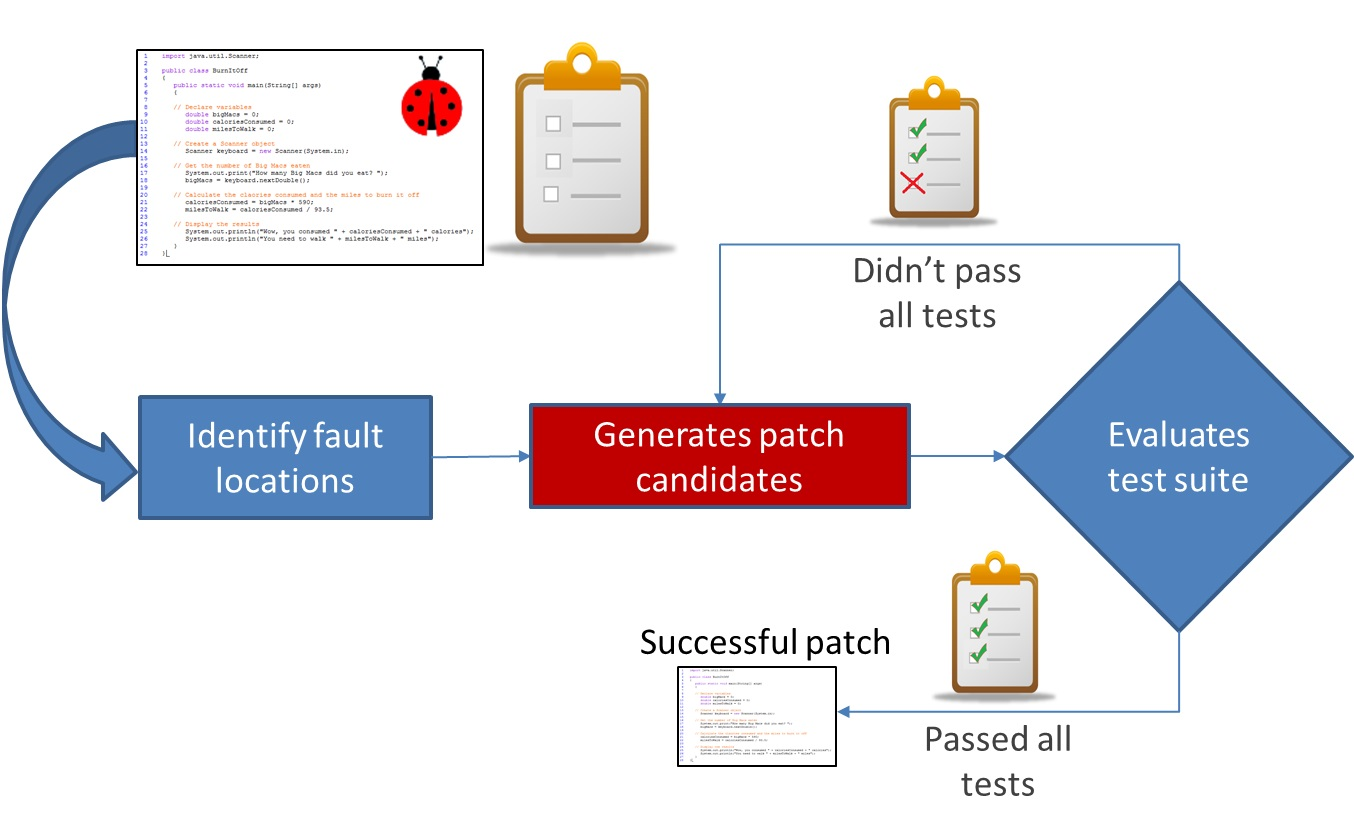
\includegraphics[scale=0.25]{Picture1}
  \caption{Generate and validate approach}
  \label{fig:generateandvalidate}
\end{figure}

The first step of this process is to localize the error to a particular statement. There is an extensive list of possible approaches in literature in order to perform this tasks \todo{List several fault loc papers}, but this paper will not focus on this particular step. Out main focus will be the next step: Generating candidate patches.\\
Once we know where the fault is located we proceed to create what we call "Candidate patches". Candidate patches are variations of the original program which may or may not be a patch for the bug(s) we are trying to fix. In order to create candidate patches we need to apply one or several mutation operators to the fault location. \\
There are several possible mutation operators that can be applied to a location in order to modify the behavior of a program. In order to analyze this we have taken mutation operators from two of the most successful approaches in program repair that use generate and validate methodology: Genprog \todo{reference to Genprog paper} is a very well known and widely used tool that modifies statements in order to create candidate patches.   PAR \todo{PAR Reference} is a successful approach that bases their patch generation technique in creating a list of commonly used templates of the most used changes that human programmers perform in order to fix bugs in their source code. We have denominated these two techniques: General mutations \todo{not sure if this is the best name for this} and Template based mutations.


\subsection{General mutations}
Claire Le Goues\todo{Refer to authors by last name only} et al. have created a very successful approach which they denominate GenProg \todo{reference to genprog}, which is a tool that modifies statements of source code in order to repair programs. A statement is the smallest standalone element that expresses some action to be carried out in a programming language. This tool is able to delete, append or replace statements in order to create candidate patches.\\
Once the tool has a set of candidate patches, it will run the test suite on each of those candidate patches. If it is able to find a candidate patch that can pass all the test cases in the test suite, that candidate patch will be considered a patch of the bug. If it is not able to pass all the test cases in the test suite, then it will go back to creating more candidate patches and will continue to do so until it reaches a stopping point, which may be a certain user defined number of generations or a user defined clock time limit.


\subsection{Template based mutations}
Dongsun Kim et al. have created the approach which they denominate Pattern-based Automatic program Repair(PAR), in which they examined a large number of human created patches and have abstracted 16 different templates to be the most commonly used changes that human programmers do in order to fix their code: \url{https://sites.google.com/site/autofixhkust/home/fix-templates}
The 16 templates which we consider in this category are the following:
\begin{enumerate}
\item Null Checker
\item Parameter Replacer
\item Method Replacer
\item Parameter Adder and Remover
\item Object Initializer
\item Sequence Exchanger
\item Range Checker
\item Collection Size Checker
\item Lower Bound Setter
\item Upper Bound Setter
\item Off-by-one Mutator
\item Class Cast Checker
\item Caster Mutator
\item Castee Mutator
\item Expression Changer
\item Expression Adder
\end{enumerate}

\section{Building the model}
The first model we built was created based on the 200 Java projects in Github with the most stars. When users star a project they are creating a bookmark for easier access, and showing appreciation to the repository maintainer for their work. Projects with more stars are more popular among the developers of Github and therefore more likely to be reviewed by other developers and have higher standards of code quality than projects with less stars.\\
Once we have checked out the 200 Java projects with the most stars, we checkout the last 100 bug fixing commits per each project. \\
In order to tell apart a bug fixing commit from a non bug fixing commit we filter them by applying a regular expression to the commit message:
\todo{fix this text}
\begin{verbatim}
    $[Ff]ix(ed|es|ing)?(\s)*([Bb]ug|[Ii]ssue|[Pp]roblem)?(s)?$
\end{verbatim}
The intuition behind this regular expression is to filter commits where their commit message includes phrases such as: "Fixed issue with variable x", "Fix for problem discussed in meeting", "Error fixed", "Fixing file bug", etc.\\
We also added two extra filters to our search: First we had commits that only modify java source code. This is with the intention of looking only into human fixing commits that fix java source code. Developers may also fix bugs in other sections of their projects, for example they may fix bugs in bash files, or xml code or any other kind of bug, and this wouldn't be relevant to our purpose of building a model that looks into the ways in which human developers fix their java code.\\
The last filter we applied to our search is to look only for the fixing commits that modify a maximum of 3 files per commit. This is for two reasons: first, we want to filter out big merges of code such as pull requests or initial commits where the commit is doing much more than just fixing a bug, which are the cases that we are interested in; and second, because these approaches usually work better when the fault is localized in a small number of locations.\\
For each of these bug fixing commits, we then checked the version of the code before the fix was performed and after the fix was performed. We refer to these versions as the "before-fix" version and the "after-fix" version.\\
We then need to know what changes are happening from the before-fix version to the after-fix version, and we need to be able to analyze how often these changes performed match the mutation operators we are analyzing in order to see what are the probabilities of each of them to happen.\\
In order to do this we used two different widely used tools for mapping changes between two versions of code: Gumtree and QACrashFix./todo{refereces to these two papers}\\
These tools create an AST representation of the program files for both the before-fix and after-fix representations of the programs for each of the files of the commit, and then use a set of heuristics to match the before-fix version with the after-fix version. Once this is done, the program's output is a set of changes needed to be performed to get from version before-fix to version after-fix.\\
We created two levels in the probabilistic model, the first one we will call the \textit{Mutation operator probabilistic model}, and the second level we will call the \textit{Replacements probabilistic model}.\\
The \textit{Mutation operator probabilistic model} is a probabilistic model that describes the probabilities to choose between the several different mutation operators in a particular fault location.\\
The \textit{Replacements probabilistic model} is the next level of the probabilistic model, which describes, if the "Replacement" mutation operator is picked, what are the probabilities of replacing one statement for another. We will explain this in detail below.\\

\begin{figure}[!h]
  \centering
    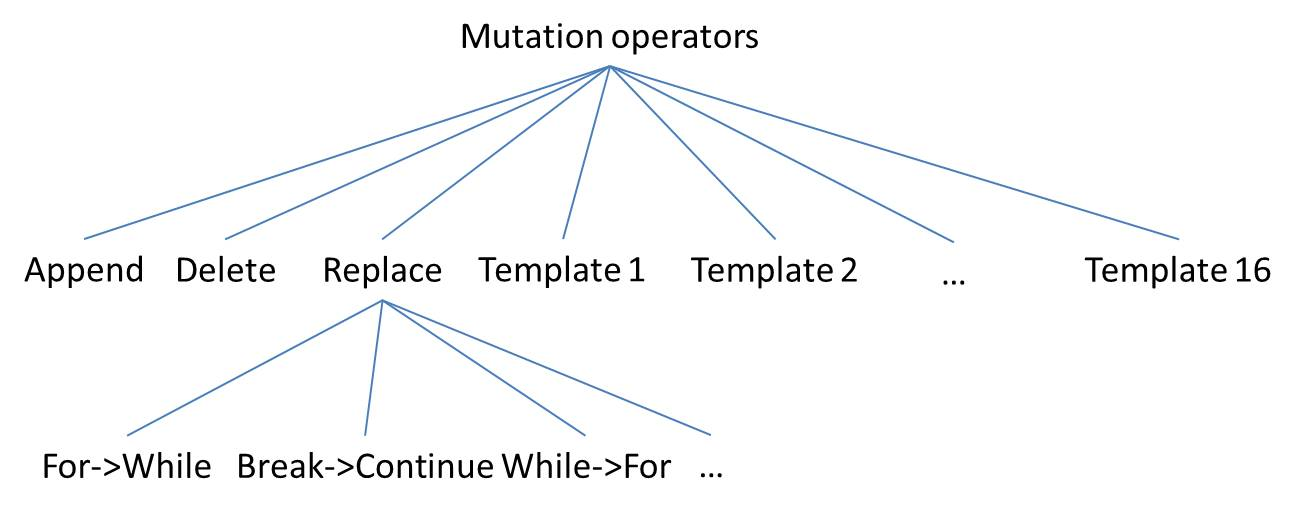
\includegraphics[scale=0.4]{Picture2}
  \caption{2 level probabilistic model}
  \label{fig:probModel}
\end{figure}

\subsection{Mutation operator probabilistic model}
In order to build the \textit{Mutation operator probabilistic model} we created a program (available at \todo{link to the github repo}) that goes through these changes and matches these changes with the mutation operators we described earlier.\\
We sum the instances of each of the appearances of the mutation operators in the lists of changes created out of the differences between the before-fix and after-fix versions of each of the files in the 100 last bug fixing commits per each of the 200 projects; and these instance sums are the data we take to create our probabilistic model.\\  


\subsection{Replacements probabilistic model}
In order to build the \textit{Replacements probabilistic model} we created a program similar to the one mentioned before (available at \todo{link to the github repo}) that goes through these changes and when it encounters a replacement mutation operator, then it looks at what kind of statement is being replaced and what kind of statement is replacing the other. We call these statements "replacee" and "replacer" accordingly.\\
We analyzed 22 different kinds of statement and the probability in which each of them replaces another. For example, what is the probability that a For loop would replace a While loop, or the probability that a Break statement would replace a Continue statement, etc.\\
Since there are 22 statement types that we analyzed and each of these 22 may replace each of these 22 statement types, we then have 484 combinations of replacement combinations. \\
It is also worth noticing that these probabilities are not reciprocal, meaning that the probability of a For loop replacing a While loop is different from the probability of a While loop replacing a For loop, and the same applies to all the different statement types.\\

\section{Sanity Check}
Section text here.

\subsection{10 fold cross validation}
Subsection text here.

\subsection{Small Example}
Subsection text here.


\section{Evaluation}
Section text here.

\section{Upgrading the model}

\subsection{Single line bugs}
Subsection text here.

\subsection{Multi line bugs}
Subsection text here.

\section{Discussion}
Section text here.



\section{Conclusion}
The conclusion goes here.




% conference papers do not normally have an appendix


% use section* for acknowledgment
\section*{Acknowledgment}


The authors would like to thank...





% trigger a \newpage just before the given reference
% number - used to balance the columns on the last page
% adjust value as needed - may need to be readjusted if
% the document is modified later
%\IEEEtriggeratref{8}
% The "triggered" command can be changed if desired:
%\IEEEtriggercmd{\enlargethispage{-5in}}

% references section

% can use a bibliography generated by BibTeX as a .bbl file
% BibTeX documentation can be easily obtained at:
% http://mirror.ctan.org/biblio/bibtex/contrib/doc/
% The IEEEtran BibTeX style support page is at:
% http://www.michaelshell.org/tex/ieeetran/bibtex/
%\bibliographystyle{IEEEtran}
% argument is your BibTeX string definitions and bibliography database(s)
%\bibliography{IEEEabrv,../bib/paper}
%
% <OR> manually copy in the resultant .bbl file
% set second argument of \begin to the number of references
% (used to reserve space for the reference number labels box)
%\begin{thebibliography}{1}

%\bibitem{IEEEhowto:kopka}

%\end{thebibliography}

\todo{Fix bibliography}
\bibliographystyle{abbrv}
\bibliography{sigproc}  % sigproc.bib is the name of the Bibliography in this case
% You must have a proper ".bib" file
%  and remember to run:
% latex bibtex latex latex
% to resolve all references



% that's all folks
\end{document}


